%======================================================================
\section{The disc-to-strip map and the layer maps}\label{sec:str}

This section constructs the planar disc-to-strip map and proves its estimate, which is
Proposition~\ref{prop:hdl-strip}. It then proves the layer step used in \Msec{sec:hdl-proof}: one ball is placed in
each layer of the handle, and the maps $\psi_i=\Phi^{-1}\circ\mathcal D^{-1}\circ E_i$ are symplectic embeddings with
pairwise disjoint images in the interior of the model (Propositions~\ref{prop:str-layer}
and~\ref{prop:str-embeddings}).

\medskip\noindent\emph{Conventions.} On $\C\ni z$ we write $\omega_\C=dx\wedge dy$ for $z=x+iy$ and $I=\pi|z|^2$;
recall $dx\wedge dy=dI\wedge d\theta$ with $\theta=\arg z/2\pi$. The strip $(0,\infty)\times(0,1)$ carries coordinates
$(x,T)$ and the area form $dx\wedge dT$. An auxiliary plane $\R^2\ni\xi=(\xi_1,\xi_2)$, identified with $\C$ by
$\xi\mapsto\xi_1+i\xi_2$, carries $d\xi=d\xi_1\wedge d\xi_2$, and $\mathrm{Rot}_\phi$ is the rotation by the angle
$\phi$. In \S\S\ref{sec:str-balls}--\ref{sec:str-embeddings} we write $\C^n=\C\times\C^m\ni(z_{\rm b},z_{\rm f})$,
$\varpi=\pi|z_{\rm b}|^2$ and $p=p(z_{\rm f})$, so that $\omega_0=\omega_\C(z_{\rm b})+\omega_V(z_{\rm f})$ and
$B(c)=\{\varpi+|p|\le c\}$, $\Bo(c)=\{\varpi+|p|<c\}$.

%----------------------------------------------------------------------
\subsection{The strip Morse functions}\label{sec:str-morse}

Fix $\delta>0$ and put $b_{\rm st}=\delta/\pi$. The strip map $\Psi_\delta$ sends the circle of area $I$ about $0$ onto a
level set $\{R_{\rm st}(x)+V_{\rm st}(T)=\mathcal E\}$ in the strip, where $R_{\rm st}$ and $V_{\rm st}$ are Morse functions
on $(0,\infty)$ and $(0,1)$ with minimum $0$. The level set of energy $\mathcal E$ lies in $\{x<\mathcal E+b_{\rm st}\}$ and
encloses area at least $\mathcal E-b_{\rm st}(\frac\pi2-1)$, so the circle of area $I$ lands in
$\{x<I+b_{\rm st}\frac\pi2\}=\{x<I+\frac\delta2\}$. Since a ball meets every base disc $\{\varpi\le c\}$ at some fibre
level, this excess must be uniform in the radius, and it is (Figure~\ref{fig:str-strip}). The map is the product $F_{\rm st}$ of signed square-root
inverses of $R_{\rm st}$ and $V_{\rm st}$, followed by two normalisations of the area density that fix every circle:
$X_{\rm st}(\xi_1)$ is the solution of $R_{\rm st}(x)=\xi_1^2$ on the side of the minimum $b_{\rm st}/2$ given by the sign
of $\xi_1$, and $Y_{\rm st}(\xi_2)$ the solution of $V_{\rm st}(T)=\xi_2^2$ on the side of $\frac12$ given by the sign of
$\xi_2$.

\begin{construction}[Strip Morse functions]\label{cons:str-morse}
\lean{SymplecticPacking.Strip.bst, SymplecticPacking.Strip.Rst, SymplecticPacking.Strip.Vst,
SymplecticPacking.Strip.Xst, SymplecticPacking.Strip.Yst, SymplecticPacking.Strip.Jst}
Let $\delta>0$ and $b_{\rm st}=\delta/\pi$. For $x>0$, $0<T<1$ and $\xi=(\xi_1,\xi_2)\in\R^2$ put
\begin{align*}
 R_{\rm st}(x)&=x+\frac{b_{\rm st}^2}{4x}-b_{\rm st}, &
 V_{\rm st}(T)&=b_{\rm st}\Big[\frac{1}{2\sqrt{T(1-T)}}-1\Big],\\
 X_{\rm st}(\xi_1)&=\tfrac12\Big[\xi_1^2+b_{\rm st}+\xi_1\sqrt{\xi_1^2+2b_{\rm st}}\Big], &
 Y_{\rm st}(\xi_2)&=\frac12+\frac{\xi_2\sqrt{\xi_2^2+2b_{\rm st}}}{2(\xi_2^2+b_{\rm st})} ,
\end{align*}
and $F_{\rm st}(\xi)=\big(X_{\rm st}(\xi_1),Y_{\rm st}(\xi_2)\big)$, $\mathcal J_{\rm st}(\xi)=X_{\rm st}'(\xi_1)\,Y_{\rm st}'(\xi_2)$.
\end{construction}

\begin{lemma}[Smooth Morse inverses]\label{lem:str-morse-inverse}
\lean{SymplecticPacking.Strip.Rst_nonneg, SymplecticPacking.Strip.Rst_eq_zero_iff,
 SymplecticPacking.Strip.Vst_nonneg, SymplecticPacking.Strip.Vst_eq_zero_iff,
 SymplecticPacking.Strip.Rst_Xst, SymplecticPacking.Strip.Vst_Yst,
 SymplecticPacking.Strip.deriv_Xst, SymplecticPacking.Strip.deriv_Yst,
 SymplecticPacking.Strip.contDiff_Xst, SymplecticPacking.Strip.contDiff_Yst,
 SymplecticPacking.Strip.Xst_bijOn, SymplecticPacking.Strip.Yst_bijOn}
\uses{cons:str-morse}
\begin{enumerate}[label=(\roman*)]
\item $R_{\rm st}\ge0$ on $(0,\infty)$ with unique zero $x=b_{\rm st}/2$, and $V_{\rm st}\ge0$ on $(0,1)$ with unique zero
$T=\frac12$.
\item $R_{\rm st}(X_{\rm st}(\xi_1))=\xi_1^2$ and $V_{\rm st}(Y_{\rm st}(\xi_2))=\xi_2^2$ for all $\xi_1,\xi_2\in\R$.
\item $X_{\rm st}$ and $Y_{\rm st}$ are smooth on $\R$, with
\[
 X_{\rm st}'(\xi_1)=\frac{\big(\xi_1+\sqrt{\xi_1^2+2b_{\rm st}}\big)^2}{2\sqrt{\xi_1^2+2b_{\rm st}}}>0,\qquad
 Y_{\rm st}'(\xi_2)=\frac{b_{\rm st}^2}{\sqrt{\xi_2^2+2b_{\rm st}}\,(\xi_2^2+b_{\rm st})^2}>0 .
\]
\item $X_{\rm st}$ is an increasing bijection $\R\to(0,\infty)$ and $Y_{\rm st}$ an increasing bijection $\R\to(0,1)$.
$F_{\rm st}$ is a smooth diffeomorphism of $\R^2$ onto $(0,\infty)\times(0,1)$ with
$F_{\rm st}^*(dx\wedge dT)=\mathcal J_{\rm st}\,d\xi$ and $R_{\rm st}\circ X_{\rm st}+V_{\rm st}\circ Y_{\rm st}=|\xi|^2$.
\end{enumerate}
\end{lemma}

\begin{proof}
(i) $R_{\rm st}(x)=(\sqrt x-b_{\rm st}/(2\sqrt x))^2$, which vanishes only at $x=b_{\rm st}/2$. Since $T(1-T)\le\frac14$ with
equality only at $T=\frac12$, $V_{\rm st}\ge0$ with unique zero $T=\frac12$.

(ii) For $x>0$, $R_{\rm st}(x)=\xi_1^2$ is equivalent to $x^2-(\xi_1^2+b_{\rm st})x+b_{\rm st}^2/4=0$, with discriminant
$(\xi_1^2+b_{\rm st})^2-b_{\rm st}^2=\xi_1^2(\xi_1^2+2b_{\rm st})$ and roots
$x_\pm=\frac12[\xi_1^2+b_{\rm st}\pm|\xi_1|\sqrt{\xi_1^2+2b_{\rm st}}]$, both positive because $x_+x_-=b_{\rm st}^2/4$.
$X_{\rm st}(\xi_1)$ is $x_+$ for $\xi_1\ge0$ and $x_-$ for $\xi_1\le0$. For the second identity write $Y_{\rm st}=\frac12+\tau$
with $\tau=\xi_2\sqrt{\xi_2^2+2b_{\rm st}}/(2(\xi_2^2+b_{\rm st}))$. Then
$\tau^2=\frac14-\frac{b_{\rm st}^2}{4(\xi_2^2+b_{\rm st})^2}<\frac14$, so $0<Y_{\rm st}<1$,
$T(1-T)=\frac14-\tau^2=b_{\rm st}^2/(4(\xi_2^2+b_{\rm st})^2)$ for $T=Y_{\rm st}(\xi_2)$, hence
$1/(2\sqrt{T(1-T)})=(\xi_2^2+b_{\rm st})/b_{\rm st}$ and $V_{\rm st}(T)=\xi_2^2$.

(iii) Smoothness holds because $\xi_1^2+2b_{\rm st}>0$ and $\xi_2^2+b_{\rm st}>0$. With $r=\sqrt{\xi_1^2+2b_{\rm st}}$,
$2X_{\rm st}'=2\xi_1+r+\xi_1^2/r=(\xi_1+r)^2/r$, and $\xi_1+r>0$ since $r>|\xi_1|$. With
$\varphi(\xi_2)=\xi_2\sqrt{\xi_2^2+2b_{\rm st}}/(\xi_2^2+b_{\rm st})$,
\[
 \varphi'(\xi_2)=\frac{(2\xi_2^2+2b_{\rm st})(\xi_2^2+b_{\rm st})-2\xi_2^2(\xi_2^2+2b_{\rm st})}
 {\sqrt{\xi_2^2+2b_{\rm st}}\,(\xi_2^2+b_{\rm st})^2}
 =\frac{2b_{\rm st}^2}{\sqrt{\xi_2^2+2b_{\rm st}}\,(\xi_2^2+b_{\rm st})^2},
\]
and $Y_{\rm st}'=\varphi'/2$.

(iv) Both maps are continuous and strictly increasing by (iii). As $\xi_1\to+\infty$, $X_{\rm st}\to\infty$; for $\xi_1<0$,
$X_{\rm st}(\xi_1)=x_-=b_{\rm st}^2/(4x_+)$ with $x_+\to\infty$ as $\xi_1\to-\infty$, so $X_{\rm st}\to0^+$. Since $\varphi$ is odd
and $\varphi^2=1-b_{\rm st}^2/(\xi_2^2+b_{\rm st})^2\to1$, $Y_{\rm st}$ increases from $0^+$ to $1^-$. Thus $F_{\rm st}$ is a
smooth bijection with Jacobian $\mathcal J_{\rm st}>0$, hence a smooth diffeomorphism by the inverse function theorem;
the last identity is (ii).
\end{proof}

%----------------------------------------------------------------------
\subsection{The strip map}\label{sec:str-map}

$F_{\rm st}$ sends circles $|\xi|^2=\mathcal E$ to level sets of $R_{\rm st}+V_{\rm st}$ but does not preserve area. Two
normalisations correct the density without moving the circles: a rotation of each circle that makes the density
constant along it, and a radial map that adjusts the enclosed area. Both are written in Cartesian coordinates, so
that smoothness at the origin is visible. They are the normalisations of Definition~\ref{def:pln-normalisations} for a single density; the
proofs are repeated here because the strip density $\mathcal J_{\rm st}$ is not constant near the origin, as setting (N)
of \S\ref{sec:pln-normalisation-maps} assumes.

\begin{definition}[Rotation and area normalisation]\label{def:str-normalisation}
\lean{SymplecticPacking.Inner.Jbar, SymplecticPacking.Inner.Bfun, SymplecticPacking.Inner.Trot,
 SymplecticPacking.Inner.Acal, SymplecticPacking.Inner.Acal_strictMono, SymplecticPacking.Inner.Acal_bijective,
 SymplecticPacking.Inner.Einv, SymplecticPacking.Inner.Darea}
Let $\mathcal J$ be a positive smooth function on $\R^2$. Put
\begin{align*}
 \bar{\mathcal J}(|\xi|^2)&=\frac1{2\pi}\int_0^{2\pi}\mathcal J(\mathrm{Rot}_\phi\xi)\,d\phi,\\
 \mathcal M(\xi)&=\frac1{2\pi}\int_0^{2\pi}(\phi-\pi)\,\mathcal J(\mathrm{Rot}_\phi\xi)\,d\phi,\\
 \mathsf T_{\mathcal J}(\xi)&=\mathrm{Rot}_{\mathcal M(\xi)/\bar{\mathcal J}(|\xi|^2)}\,\xi .
\end{align*}
and $\mathfrak a_{\mathcal J}(\mathcal E)=\int_{|\xi|^2\le\mathcal E}\mathcal J\,d\xi$ for $\mathcal E\ge0$. In polar coordinates
$\mathfrak a_{\mathcal J}(\mathcal E)=\int_0^{\sqrt{\mathcal E}}\int_0^{2\pi}\mathcal J\,d\psi\,r\,dr
=\int_0^{\sqrt{\mathcal E}}2\pi r\bar{\mathcal J}(r^2)\,dr=\pi\int_0^{\mathcal E}\bar{\mathcal J}(t)\,dt$ with $\bar{\mathcal J}>0$, so
$\mathfrak a_{\mathcal J}$ is continuous and strictly increasing with $\mathfrak a_{\mathcal J}(0)=0$. If
$\mathfrak a_{\mathcal J}(\mathcal E)\to\infty$ as $\mathcal E\to\infty$, it is a bijection of $[0,\infty)$; then let
$\mathcal E_{\mathcal J}=\mathfrak a_{\mathcal J}^{-1}$ and, for $z\in\C$ with $I=\pi|z|^2$,
\[
 \mathsf D_{\mathcal J}(z)=\sqrt{\pi\,\mathcal E_{\mathcal J}(I)/I}\;z\quad(z\ne0),\qquad \mathsf D_{\mathcal J}(0)=0 .
\]
\end{definition}

\begin{lemma}[Normalisation]\label{lem:str-normalisation}
\lean{SymplecticPacking.Inner.Trot_bijective, SymplecticPacking.Inner.Trot_det,
 SymplecticPacking.Inner.Darea_bijective, SymplecticPacking.Inner.norm_Darea_sq,
 SymplecticPacking.Inner.Darea_pullback, SymplecticPacking.Strip.normalize_general}
\uses{def:str-normalisation}
Let $\mathcal J$ be a positive smooth function on $\R^2$.
\begin{enumerate}[label=(\roman*)]
\item $\mathsf T_{\mathcal J}$ is a smooth diffeomorphism of $\R^2$ which maps every circle
$\{|\xi|=r\}$ onto itself, and $\mathsf T_{\mathcal J}^*\big(\bar{\mathcal J}(|\xi|^2)\,d\xi\big)=\mathcal J\,d\xi$.
\item If $\mathfrak a_{\mathcal J}(\mathcal E)\to\infty$, then $\mathsf D_{\mathcal J}$ is a smooth
diffeomorphism $\C\to\R^2$ with $|\mathsf D_{\mathcal J}(z)|^2=\mathcal E_{\mathcal J}(\pi|z|^2)$ and
$\mathsf D_{\mathcal J}^*\big(\bar{\mathcal J}(|\xi|^2)\,d\xi\big)=\omega_\C$.
\item If $\mathfrak a_{\mathcal J}(\mathcal E)\to\infty$ and $F\colon\R^2\to U$ is a smooth
diffeomorphism onto an open set $U\subset\R^2$ with $F^*(dx\wedge dT)=\mathcal J\,d\xi$, then
$F\circ\mathsf T_{\mathcal J}^{-1}\circ\mathsf D_{\mathcal J}\colon\C\to U$ is a smooth
diffeomorphism which pulls $dx\wedge dT$ back to $\omega_\C$ and maps the circle $\{\pi|z|^2=I\}$ onto
$F(\{|\xi|^2=\mathcal E_{\mathcal J}(I)\})$.
\end{enumerate}
\end{lemma}

\begin{proof}
If $g(\phi,\xi)$ is smooth on $\R\times\R^2$, then
$\xi\mapsto\int_0^{2\pi}g(\phi,\xi)\,d\phi$ is smooth, by differentiation under
the integral sign. Thus $\mathcal M$ and
$\xi\mapsto\bar{\mathcal J}(|\xi|^2)$ are smooth, and $\bar{\mathcal J}>0$.
A smooth bijection with nowhere vanishing Jacobian has a smooth inverse by the
inverse function theorem.

(i) Fix $r>0$ and put $\mathcal J_r(\psi)=\mathcal J(re^{i\psi})$, a $2\pi$-periodic function. Then
$\mathcal M(re^{i\psi})=\frac1{2\pi}\int_0^{2\pi}(\phi-\pi)\mathcal J_r(\psi+\phi)\,d\phi$, and integration by parts gives
\[
 \partial_\psi\mathcal M(re^{i\psi})=\frac1{2\pi}\Big[(\phi-\pi)\mathcal J_r(\psi+\phi)\Big]_{\phi=0}^{2\pi}
 -\frac1{2\pi}\int_0^{2\pi}\mathcal J_r(\psi+\phi)\,d\phi
 =\mathcal J_r(\psi)-\bar{\mathcal J}(r^2).
\]
So $\mathsf T_{\mathcal J}(re^{i\psi})=re^{i\Theta(\psi)}$ with $\Theta=\psi+\mathcal M/\bar{\mathcal J}$,
$\Theta'=\mathcal J/\bar{\mathcal J}>0$ and $\Theta(\psi+2\pi)=\Theta(\psi)+2\pi$: $\mathsf T_{\mathcal J}$ maps each circle
diffeomorphically onto itself, $\mathsf T_{\mathcal J}(0)=0$, and $\mathsf T_{\mathcal J}$ is a bijection of $\R^2$. The angle
$\vartheta=\mathcal M/\bar{\mathcal J}(|\xi|^2)$ is smooth, so $\mathsf T_{\mathcal J}(\xi)=\mathrm{Rot}_{\vartheta(\xi)}\xi$ is
smooth. In polar coordinates, since $\bar{\mathcal J}$ is radial and $\mathsf T_{\mathcal J}$ preserves $r$,
$\mathsf T_{\mathcal J}^*(\bar{\mathcal J}\,r\,dr\wedge d\psi)=\bar{\mathcal J}\,r\,dr\wedge(\partial_r\Theta\,dr+\Theta'\,d\psi)
=\mathcal J\,r\,dr\wedge d\psi$ off the origin. Hence $\det D\mathsf T_{\mathcal J}=\mathcal J/\bar{\mathcal J}>0$ off the origin, and at
the origin by continuity, so $\mathsf T_{\mathcal J}$ is a smooth diffeomorphism.

(ii) Put
\[
 G(\xi)=\int_0^1\bar{\mathcal J}\big(t|\xi|^2\big)\,dt
 =\frac1{2\pi}\int_0^1\!\!\int_0^{2\pi}2r\,\mathcal J\big(\mathrm{Rot}_\phi(r\xi)\big)\,d\phi\,dr ,
\]
a smooth positive function of $\xi$ (the same argument as above, over the compact set $[0,1]\times[0,2\pi]$), with
$\pi|\xi|^2G(\xi)=\mathfrak a_{\mathcal J}(|\xi|^2)$ by the polar formula of Definition~\ref{def:str-normalisation}. The smooth map
$\mathsf D'(\xi)=\sqrt{G(\xi)}\,\xi$ preserves the argument and satisfies $\pi|\mathsf D'(\xi)|^2=\mathfrak a_{\mathcal J}(|\xi|^2)$;
since $\mathfrak a_{\mathcal J}$ is a bijection of $[0,\infty)$, $\mathsf D'$ is a bijection of $\R^2$, and it is the inverse of
$\mathsf D_{\mathcal J}$: if $I=\pi|\mathsf D'(\xi)|^2$ then $\mathcal E_{\mathcal J}(I)=|\xi|^2$ and
$\mathsf D_{\mathcal J}(\mathsf D'(\xi))=\sqrt{\pi|\xi|^2/I}\,\sqrt{G(\xi)}\,\xi=\xi$. In polar coordinates, with
$\mathcal E=|\xi|^2$, $\mathsf D'$ preserves the angle $\psi$ and sends $\mathcal E$ to $I=\mathfrak a_{\mathcal J}(\mathcal E)$, so off
the origin
\[
 (\mathsf D')^*\omega_\C=(\mathsf D')^*\Big(\frac{dI\wedge d\psi}{2\pi}\Big)
 =\frac{\pi\bar{\mathcal J}(\mathcal E)\,d\mathcal E\wedge d\psi}{2\pi}
 =\bar{\mathcal J}(|\xi|^2)\,r\,dr\wedge d\psi=\bar{\mathcal J}(|\xi|^2)\,d\xi .
\]
Thus $\det D\mathsf D'=\bar{\mathcal J}(|\xi|^2)>0$, also at the origin by continuity, and $\mathsf D'$ is a smooth
diffeomorphism. Hence so is $\mathsf D_{\mathcal J}=(\mathsf D')^{-1}$, and
$\mathsf D_{\mathcal J}^*(\bar{\mathcal J}\,d\xi)=\omega_\C$. Finally
$|\mathsf D_{\mathcal J}(z)|^2=(\pi\mathcal E_{\mathcal J}(I)/I)|z|^2=\mathcal E_{\mathcal J}(I)$.

(iii) By (i) and (ii) the composite is a smooth diffeomorphism onto $F(\R^2)=U$, and
$(F\circ\mathsf T_{\mathcal J}^{-1}\circ\mathsf D_{\mathcal J})^*(dx\wedge dT)
=\mathsf D_{\mathcal J}^*(\mathsf T_{\mathcal J}^{-1})^*(\mathcal J\,d\xi)=\mathsf D_{\mathcal J}^*(\bar{\mathcal J}\,d\xi)=\omega_\C$.
$\mathsf D_{\mathcal J}$ maps $\{\pi|z|^2=I\}$ onto $\{|\xi|^2=\mathcal E_{\mathcal J}(I)\}$, which $\mathsf T_{\mathcal J}^{-1}$
preserves.
\end{proof}

We apply this to $\mathcal J=\mathcal J_{\rm st}$ and write $\bar{\mathcal J}_{\rm st}$ and
$\mathfrak a_{\rm st}=\mathfrak a_{\mathcal J_{\rm st}}$. The next lemma contains the area facts behind the strip estimate.

\begin{lemma}[Sublevel sets and area]\label{lem:str-area}
\lean{SymplecticPacking.Strip.width_sublevel, SymplecticPacking.Strip.lt_of_Rst_le,
 SymplecticPacking.Strip.sublevel_empty, SymplecticPacking.Strip.integral_Vst,
 SymplecticPacking.Strip.Ast_eq_integral, SymplecticPacking.Strip.Fst_bijOn, SymplecticPacking.Strip.Fst_det, SymplecticPacking.Strip.level_Fst, SymplecticPacking.Strip.Ast_ge,
 SymplecticPacking.Strip.Ast_Est, SymplecticPacking.Strip.gAcal_strictMono, SymplecticPacking.Strip.gAcal_zero, SymplecticPacking.Strip.Ast_tendsto, SymplecticPacking.Strip.gAcal_hasDerivAt}
\uses{cons:str-morse, lem:str-morse-inverse, def:str-normalisation}
Let $b_{\rm st}=\delta/\pi$.
\begin{enumerate}[label=(\roman*)]
\item For $c\ge0$, $\{x>0:R_{\rm st}(x)\le c\}=[x_-(c),x_+(c)]$ with
$x_\pm(c)=\frac12\big[c+b_{\rm st}\pm\sqrt{c(c+2b_{\rm st})}\big]$. Its length is $\sqrt{c(c+2b_{\rm st})}\ge c$, and
$0<x_-(c)\le x_+(c)<c+b_{\rm st}$. For $c<0$ the set is empty.
\item $\int_0^1V_{\rm st}(T)\,dT=b_{\rm st}(\frac\pi2-1)$.
\item $\mathfrak a_{\rm st}(\mathcal E)$ is the $dx\,dT$-area of $\{(x,T):R_{\rm st}(x)+V_{\rm st}(T)\le\mathcal E\}$, and
$\mathfrak a_{\rm st}(\mathcal E)\ge\mathcal E-b_{\rm st}(\frac\pi2-1)$.
\item $\mathfrak a_{\rm st}$ is a continuous strictly increasing bijection of $[0,\infty)$, with
$\mathfrak a_{\rm st}'(\mathcal E)=\pi\bar{\mathcal J}_{\rm st}(\mathcal E)>0$.
\end{enumerate}
\end{lemma}

\begin{proof}
(i) This is the computation in the proof of Lemma~\ref{lem:str-morse-inverse}(ii) with $\xi_1^2=c$:
$x_+-x_-=\sqrt{c(c+2b_{\rm st})}\ge c$, and $\sqrt{c(c+2b_{\rm st})}<c+b_{\rm st}$ because
$(c+b_{\rm st})^2-c(c+2b_{\rm st})=b_{\rm st}^2>0$; this gives $x_->0$ and $x_+<c+b_{\rm st}$. For $c<0$ the set is empty since
$R_{\rm st}\ge0$.
(ii) $\int_0^1dT/\sqrt{T(1-T)}=\pi$ (substitute $T=\sin^2\phi$).
(iii) By Lemma~\ref{lem:str-morse-inverse}(iv), $F_{\rm st}$ is a diffeomorphism onto the strip with Jacobian $\mathcal J_{\rm st}$
which maps $\{|\xi|^2\le\mathcal E\}$ onto $\{R_{\rm st}+V_{\rm st}\le\mathcal E\}$; the change of variables formula gives
the first claim. By Fubini and (i),
\[
 \mathfrak a_{\rm st}(\mathcal E)=\int_0^1\big|\{x>0:R_{\rm st}(x)\le\mathcal E-V_{\rm st}(T)\}\big|\,dT
 \ge\int_0^1\big(\mathcal E-V_{\rm st}(T)\big)_+\,dT\ge\mathcal E-b_{\rm st}\big(\tfrac\pi2-1\big).
\]
(iv) By Definition~\ref{def:str-normalisation}, $\mathfrak a_{\rm st}(\mathcal E)=\pi\int_0^{\mathcal E}\bar{\mathcal J}_{\rm st}$ is
continuous and strictly increasing from $0$, with the stated derivative; by (iii) it tends to $\infty$.
\end{proof}

\begin{construction}[The strip map]\label{cons:str-map}
\lean{SymplecticPacking.Strip.Ast, SymplecticPacking.Strip.psiStrip}
\uses{cons:str-morse, lem:str-morse-inverse, def:str-normalisation, lem:str-area}
For $\delta>0$ let $\mathsf T_{\rm st}=\mathsf T_{\mathcal J_{\rm st}}$, $\mathcal E_{\rm st}=\mathfrak a_{\rm st}^{-1}$ (defined on
$[0,\infty)$ by Lemma~\ref{lem:str-area}(iv)) and $\mathsf D_{\rm st}=\mathsf D_{\mathcal J_{\rm st}}$, and define
\[
 \Psi_\delta=F_{\rm st}\circ\mathsf T_{\rm st}^{-1}\circ\mathsf D_{\rm st}\colon\C\to(0,\infty)\times(0,1),\qquad
 \Psi_\delta(z)=(x,T).
\]
\end{construction}

\begin{proposition}[Disc-to-strip map]\label{prop:str-strip}
\lean{SymplecticPacking.Strip.psiStrip_smooth, SymplecticPacking.Strip.psiStrip_symplectic,
 SymplecticPacking.Strip.psiStrip_level, SymplecticPacking.Strip.psiStrip_bijOn,
 SymplecticPacking.Strip.psiStrip_x_pos, SymplecticPacking.Strip.psiStrip_x_lt,
 SymplecticPacking.Strip.psiStrip_mem, SymplecticPacking.Strip.x_lower_margin,
 SymplecticPacking.Strip.T_margin}
\uses{cons:str-map, lem:str-normalisation, lem:str-area, lem:str-morse-inverse}
Let $\delta>0$ and $b_{\rm st}=\delta/\pi$. Then:
\begin{enumerate}[label=(\roman*)]
\item $\Psi_\delta$ is a smooth diffeomorphism of $\C$ onto $(0,\infty)\times(0,1)$ with
$\Psi_\delta^*(dx\wedge dT)=\omega_\C$;
\item $R_{\rm st}(x)+V_{\rm st}(T)=\mathcal E_{\rm st}(\pi|z|^2)$ for $(x,T)=\Psi_\delta(z)$;
\item for every $z\in\C$, with $(x,T)=\Psi_\delta(z)$,
\begin{equation}\label{eq:str-x-bound}
 0<x<\pi|z|^2+\frac\delta2,\qquad 0<T<1;
\end{equation}
\item for $I_{\max}\ge0$, $\mathcal E_{\max}=I_{\max}+b_{\rm st}(\frac\pi2-1)$ and $\pi|z|^2\le I_{\max}$,
\[
 x\ge\tfrac12\Big[\mathcal E_{\max}+b_{\rm st}-\sqrt{\mathcal E_{\max}(\mathcal E_{\max}+2b_{\rm st})}\Big]>0,\qquad
 \big|T-\tfrac12\big|\le\tfrac12\sqrt{1-(1+\mathcal E_{\max}/b_{\rm st})^{-2}}<\tfrac12 .
\]
\end{enumerate}
In particular $\Psi_\delta$ has the properties stated in Proposition~\ref{prop:hdl-strip}.
\end{proposition}

\begin{figure}[ht]
\centering
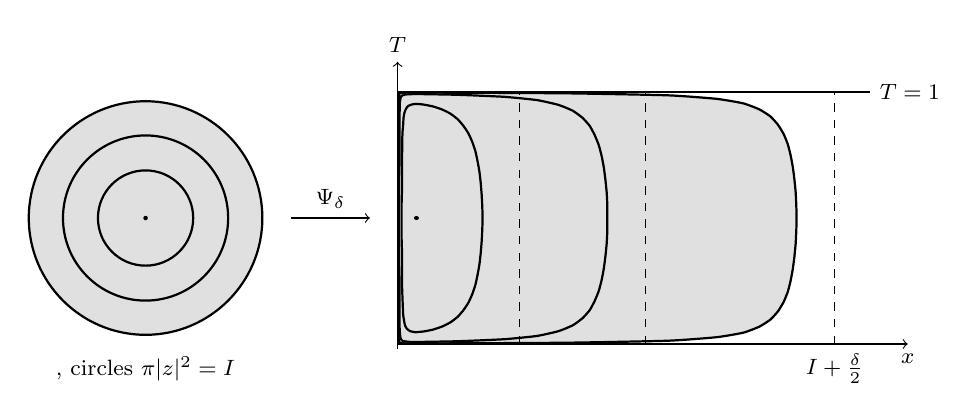
\begin{tikzpicture}[font=\footnotesize]
 \begin{scope}[scale=2.4]
  \fill[black!12] (0,0) circle (0.618);
  \draw[thick] (0,0) circle (0.252);
  \draw[thick] (0,0) circle (0.437);
  \draw[thick] (0,0) circle (0.618);
  \fill (0,0) circle (0.012);
  \node at (0,-0.8) {$\C$, circles $\pi|z|^2=I$};
 \end{scope}
 \draw[->] (1.85,0) -- node[above] {$\Psi_\delta$} (2.85,0);
 \begin{scope}[shift={(3.2,-1.6)},x=4cm,y=3.2cm]
  \fill[black!12] plot[smooth cycle,tension=0.3] coordinates {(0.060,0.002) (0.529,0.005) (0.858,0.013) (1.013,0.027) (1.098,0.045) (1.149,0.069) (1.184,0.097) (1.208,0.130) (1.226,0.167) (1.239,0.207) (1.248,0.251) (1.255,0.298) (1.260,0.346) (1.264,0.397) (1.266,0.448) (1.267,0.500) (1.266,0.552) (1.264,0.603) (1.260,0.654) (1.255,0.702) (1.248,0.749) (1.239,0.793) (1.226,0.833) (1.208,0.870) (1.184,0.903) (1.149,0.931) (1.098,0.955) (1.013,0.973) (0.858,0.987) (0.529,0.995) (0.060,0.998) (0.009,0.996) (0.005,0.989) (0.004,0.977) (0.003,0.960) (0.003,0.937) (0.003,0.910) (0.003,0.879) (0.003,0.843) (0.003,0.803) (0.003,0.760) (0.003,0.714) (0.003,0.666) (0.003,0.616) (0.003,0.565) (0.003,0.513) (0.003,0.461) (0.003,0.409) (0.003,0.359) (0.003,0.310) (0.003,0.262) (0.003,0.218) (0.003,0.177) (0.003,0.139) (0.003,0.105) (0.003,0.076) (0.003,0.051) (0.003,0.031) (0.004,0.016) (0.006,0.006) (0.026,0.002)};
  \draw[thick] plot[smooth cycle,tension=0.3] coordinates {(0.060,0.047) (0.084,0.050) (0.112,0.057) (0.141,0.069) (0.168,0.086) (0.191,0.108) (0.209,0.134) (0.225,0.164) (0.237,0.197) (0.247,0.234) (0.254,0.274) (0.260,0.316) (0.264,0.360) (0.267,0.406) (0.269,0.453) (0.270,0.500) (0.269,0.547) (0.267,0.594) (0.264,0.640) (0.260,0.684) (0.254,0.726) (0.247,0.766) (0.237,0.803) (0.225,0.836) (0.209,0.866) (0.191,0.892) (0.168,0.914) (0.141,0.931) (0.112,0.943) (0.084,0.950) (0.060,0.953) (0.047,0.951) (0.034,0.945) (0.027,0.934) (0.022,0.918) (0.019,0.898) (0.018,0.873) (0.016,0.844) (0.015,0.812) (0.015,0.776) (0.014,0.737) (0.014,0.695) (0.014,0.651) (0.014,0.606) (0.013,0.559) (0.013,0.512) (0.013,0.464) (0.013,0.417) (0.014,0.371) (0.014,0.327) (0.014,0.284) (0.014,0.244) (0.015,0.206) (0.016,0.172) (0.017,0.141) (0.018,0.114) (0.021,0.091) (0.024,0.073) (0.030,0.060) (0.040,0.051) (0.055,0.047)};
  \draw[dashed] (0.388,0) -- (0.388,1);
  \draw[thick] plot[smooth cycle,tension=0.3] coordinates {(0.060,0.008) (0.191,0.011) (0.339,0.019) (0.443,0.032) (0.511,0.051) (0.556,0.074) (0.587,0.102) (0.610,0.134) (0.626,0.171) (0.639,0.211) (0.648,0.254) (0.655,0.300) (0.660,0.348) (0.664,0.398) (0.666,0.449) (0.666,0.500) (0.666,0.551) (0.664,0.602) (0.660,0.652) (0.655,0.700) (0.648,0.746) (0.639,0.789) (0.626,0.829) (0.610,0.866) (0.587,0.898) (0.556,0.926) (0.511,0.949) (0.443,0.968) (0.339,0.981) (0.191,0.989) (0.060,0.992) (0.024,0.990) (0.012,0.984) (0.009,0.972) (0.007,0.955) (0.007,0.932) (0.006,0.905) (0.006,0.874) (0.006,0.839) (0.006,0.799) (0.006,0.757) (0.006,0.712) (0.005,0.664) (0.005,0.615) (0.005,0.564) (0.005,0.513) (0.005,0.461) (0.005,0.410) (0.005,0.360) (0.005,0.312) (0.006,0.265) (0.006,0.221) (0.006,0.181) (0.006,0.143) (0.006,0.110) (0.006,0.081) (0.007,0.056) (0.008,0.036) (0.010,0.022) (0.016,0.012) (0.043,0.008)};
  \draw[dashed] (0.788,0) -- (0.788,1);
  \draw[thick] plot[smooth cycle,tension=0.3] coordinates {(0.060,0.002) (0.529,0.005) (0.858,0.013) (1.013,0.027) (1.098,0.045) (1.149,0.069) (1.184,0.097) (1.208,0.130) (1.226,0.167) (1.239,0.207) (1.248,0.251) (1.255,0.298) (1.260,0.346) (1.264,0.397) (1.266,0.448) (1.267,0.500) (1.266,0.552) (1.264,0.603) (1.260,0.654) (1.255,0.702) (1.248,0.749) (1.239,0.793) (1.226,0.833) (1.208,0.870) (1.184,0.903) (1.149,0.931) (1.098,0.955) (1.013,0.973) (0.858,0.987) (0.529,0.995) (0.060,0.998) (0.009,0.996) (0.005,0.989) (0.004,0.977) (0.003,0.960) (0.003,0.937) (0.003,0.910) (0.003,0.879) (0.003,0.843) (0.003,0.803) (0.003,0.760) (0.003,0.714) (0.003,0.666) (0.003,0.616) (0.003,0.565) (0.003,0.513) (0.003,0.461) (0.003,0.409) (0.003,0.359) (0.003,0.310) (0.003,0.262) (0.003,0.218) (0.003,0.177) (0.003,0.139) (0.003,0.105) (0.003,0.076) (0.003,0.051) (0.003,0.031) (0.004,0.016) (0.006,0.006) (0.026,0.002)};
  \draw[dashed] (1.388,0) -- (1.388,1);
  \draw (0,0) -- (1.5,0);
  \draw (0,1) -- (1.5,1) node[right] {$T=1$};
  \draw[->] (0,-0.02) -- (0,1.12) node[above] {$T$};
  \draw[->] (0,0) -- (1.62,0) node[below] {$x$};
  \fill (0.06,0.5) circle (0.008);
  \node[below] at (1.388,0) {$I+\frac\delta2$};
 \end{scope}
\end{tikzpicture}
\caption{The disc-to-strip map $\Psi_\delta$ of Proposition~\ref{prop:str-strip}: computed level sets for $b_{\rm st}=\delta/\pi=0.12$
and $I=0.2,\,0.6,\,1.2$. The circle of area $I$ goes to the level set $\{R_{\rm st}+V_{\rm st}=\mathcal E_{\rm st}(I)\}$, which
encloses area $I$ and lies in $\{x<I+\frac\delta2\}$ (dashed lines); the dot is the common minimum $(b_{\rm st}/2,\frac12)$. The axes $x$ and $T$ have different scales.}
\label{fig:str-strip}
\end{figure}

\begin{proof}
(i), (ii) Apply Lemma~\ref{lem:str-normalisation}(iii) to the smooth positive density
$\mathcal J_{\rm st}$ and $F_{\rm st}$. The latter is given by Lemma~\ref{lem:str-morse-inverse}(iv),
and $\mathfrak a_{\rm st}\to\infty$ by Lemma~\ref{lem:str-area}(iii). The level
identity follows from $R_{\rm st}\circ X_{\rm st}+V_{\rm st}\circ Y_{\rm st}=|\xi|^2$.
(iii) Let $I=\pi|z|^2$ and $\mathcal E=\mathcal E_{\rm st}(I)$. By Lemma~\ref{lem:str-area}(iii),
$I=\mathfrak a_{\rm st}(\mathcal E)\ge\mathcal E-b_{\rm st}(\frac\pi2-1)$. By (ii) and $V_{\rm st}\ge0$, $R_{\rm st}(x)\le\mathcal E$, so by
Lemma~\ref{lem:str-area}(i)
\[
 x\le x_+(\mathcal E)<\mathcal E+b_{\rm st}\le I+b_{\rm st}\tfrac\pi2=I+\tfrac\delta2 .
\]
Positivity of $x$ and $0<T<1$ hold because $\Psi_\delta$ takes values in the strip.
(iv) Let $\mathcal E=\mathcal E_{\rm st}(\pi|z|^2)$. Since $\mathcal E_{\rm st}$ is increasing, $\mathcal E\le\mathcal E_{\rm st}(I_{\max})$, and
$I_{\max}=\mathfrak a_{\rm st}(\mathcal E_{\rm st}(I_{\max}))\ge\mathcal E_{\rm st}(I_{\max})-b_{\rm st}(\frac\pi2-1)$ by
Lemma~\ref{lem:str-area}(iii); so $\mathcal E\le\mathcal E_{\max}$. By (ii), $R_{\rm st}(x)\le\mathcal E_{\max}$ and
$V_{\rm st}(T)\le\mathcal E_{\max}$. The first bound is $x\ge x_-(\mathcal E_{\max})>0$ (Lemma~\ref{lem:str-area}(i)). The second
says $2\sqrt{T(1-T)}\ge(1+\mathcal E_{\max}/b_{\rm st})^{-1}$, i.e.\
$(T-\frac12)^2=\frac14-T(1-T)\le\frac14\big[1-(1+\mathcal E_{\max}/b_{\rm st})^{-2}\big]$.
\end{proof}

%----------------------------------------------------------------------
\subsection{Enlarged capacities and the ball estimate}\label{sec:str-balls}

Throughout the remaining layer construction we work in the situation of \Mref{Theorem}{thm:mech-packing} with $n\ge3$: a model input
(\Mref{Definition}{def:mech-model}) of rank $m=n-1$ with handle data (\Mref{Definition}{def:hdl-handle-data}), capacities $a_1,\dots,a_k>0$ with
$\{p\in\R^m_{\ge0}:|p|\le a_i\}\subset\tau_\Delta\Delta$ for some $\tau_\Delta<1$, a function $P$ and a comparison datum
$(K,q)$ with gap $\gamma>0$, and capacities $\rho_i<a_i$. The outer faces of $\Delta$ are $\{\langle b_\nu,p\rangle=\ell_\nu\}$,
$1\le\nu\le N$, with $\ell_\nu>0$. The caps $h_i$ are those of (\Mnum{eq:hdl-caps}) with $\rho_i^\sharp=\hat\rho_i$
($\hat\rho_i$ is defined in Definition~\ref{def:str-enlarged} below). By \Mref{Proposition}{prop:hdl-layers}(i), each $h_i$
is smooth on $\R^m$ and
\begin{equation}\label{eq:str-cap}
 0\le h_i(p),\qquad (a_i+\hat\rho_i)/2-|p|\le h_i(p)\qquad(p\in\R^m).
\end{equation}

\begin{lemma}[Interior of the fibre polytope]\label{lem:str-int}
\uses{M-def:mech-model}
Let $V_\Delta=\{w\in\C^m:\langle b_\nu,p(w)\rangle\le\ell_\nu\ \text{for all }\nu\}$. Then
\begin{equation}\label{eq:str-int}
 \operatorname{int}V_\Delta=\{w\in\C^m:\langle b_\nu,p(w)\rangle<\ell_\nu\ \text{for all }\nu\},
\end{equation}
and $\{w:|p(w)|\le a_i\}\subset\operatorname{int}V_\Delta$ for $1\le i\le k$.
\end{lemma}

\begin{proof}
The right side of \eqref{eq:str-int} is open and contained in $V_\Delta$. If $\langle b_\nu,p(w)\rangle=\ell_\nu>0$ for some $\nu$,
then $\langle b_\nu,p((1+t)w)\rangle=(1+t)^2\ell_\nu>\ell_\nu$ for $t>0$, so $w$ is not an interior point. If $|p(w)|\le a_i$, then
$p(w)\in\tau_\Delta\Delta$, so $\langle b_\nu,p(w)\rangle\le\tau_\Delta\ell_\nu<\ell_\nu$ for all $\nu$.
\end{proof}

The margin $a_i-\rho_i=2\delta_i$ gives nested source balls and a positive gap between
the strip image and the cap. We use strip parameter $\varepsilon_i=\delta_i/8$, whose excess
is less than $\delta_i/16$.

\begin{definition}[Enlarged capacities]\label{def:str-enlarged}
\lean{SymplecticPacking.HighDim.RawToricModel.packingSource,
SymplecticPacking.Branch2.CubicData.rhoBar, SymplecticPacking.Branch2.CubicData.deltaStrip,
SymplecticPacking.Branch2.CubicData.rhoHat}
For $1\le i\le k$ put
\[
 \delta_i=\frac{a_i-\rho_i}2,\qquad
 \bar\rho_i=a_i-\frac34\delta_i,\qquad \hat\rho_i=a_i-\frac{\delta_i}2 .
\]
Here $\bar\rho_i$ is the closed enlarged source capacity and $\hat\rho_i$ the open domain capacity, and
$\rho_i<\frac{\rho_i+a_i}2=a_i-\delta_i<\bar\rho_i<\hat\rho_i<a_i$. Put
$\varepsilon_i=(a_i-\hat\rho_i)/4=\delta_i/8$; the $i$-th ball is placed by $\Psi_{\varepsilon_i}$.
In the four-dimensional branch (\S\ref{sec:shd-four}) the same letters denote different values:
there $\bar\rho_i=(\rho_i+a_i)/2=a_i-\delta_i$, $\hat\rho_i=a_i-\frac34\delta_i$, and the $i$-th ball is placed by
$\Psi_{\delta_i}$ (Proposition~\ref{prop:shd4-maps}). The two branches never occur together, and each section states which
values it uses.
\end{definition}

\begin{lemma}[Ball estimate]\label{lem:str-ball}
\lean{SymplecticPacking.HighDim.ToricPackingStages.thinPlanar_bound,
SymplecticPacking.HighDim.ToricPackingStages.smoothCap_ge,
SymplecticPacking.Strip.Cubic.x_lt_hi}
\uses{prop:str-strip, def:str-enlarged, lem:str-int, M-prop:hdl-layers}
Let $1\le i\le k$, $(z_{\rm b},z_{\rm f})\in\C\times\C^m$, $\varpi=\pi|z_{\rm b}|^2$, $p=p(z_{\rm f})$, and let $x$ be the first
component of $\Psi_{\varepsilon_i}(z_{\rm b})$.
\begin{enumerate}[label=(\alph*)]
\item If $\varpi+|p|\le a_i-\delta_i$, then
\begin{equation}\label{eq:str-ball}
 x<\varpi+\frac{\delta_i}{16}\le a_i-|p|-\frac{15\delta_i}{16}
 \le h_i(p)-\frac{11\delta_i}{16}<h_i(p)-\frac{\delta_i}2 .
\end{equation}
\item If $\varpi+|p|\le\bar\rho_i$, then $x<a_i-|p|-\frac{11\delta_i}{16}\le h_i(p)-\frac{7\delta_i}{16}<h_i(p)-\frac{\delta_i}4$.
\item If $\varpi+|p|<\hat\rho_i$, then $x<a_i-|p|-\frac{7\delta_i}{16}\le h_i(p)-\frac{3\delta_i}{16}<h_i(p)$.
\end{enumerate}
In each case $|p|<a_i$, hence $z_{\rm f}\in\operatorname{int}V_\Delta$.
\end{lemma}

\begin{proof}
By \eqref{eq:str-x-bound}, $x<\varpi+\varepsilon_i/2=\varpi+\delta_i/16$. (a) $\varpi\le a_i-\delta_i-|p|=a_i-|p|-\delta_i$. (b)
$\varpi\le\bar\rho_i-|p|=a_i-|p|-\frac34\delta_i$. (c) $\varpi<\hat\rho_i-|p|=a_i-|p|-\frac12\delta_i$. In each case the
cap comparison is \eqref{eq:str-cap} in the form $a_i-\delta_i/4-|p|\le h_i(p)$. Finally $|p|\le\varpi+|p|<a_i$, and the last
assertion is Lemma~\ref{lem:str-int}.
\end{proof}

The base factor is placed by $\Psi_{\varepsilon_i}$, which is not toric, and the fibre level $p$ enters only through the bound
$x<h_i(p)$.

%----------------------------------------------------------------------
\subsection{Layer coordinates}\label{sec:str-layer-coords}

We recall the objects of \Msec{sec:hdl} and \S\ref{sec:shd} used here. In the product coordinates of
\Mref{Definition}{def:hdl-handle-data}, $E|_{\mathcal A^+}\cong\mathcal A^+\times\C^m$ with base coordinates $(s,v)$ and fibre
coordinate $w$, and $\omega_V=\sum_jdp_j\wedge d\theta_j$. The one-form $\beta$ equals $b(v)\,dv$ on $\mathcal A^+$, where $b\ge0$
is smooth, $b>0$ exactly on $(v_-,v_+)$ and $\int b=1$. The layer intervals $I_j=[l_j,r_j]\subset(0,1)$,
$1\le j\le k$, and the residual interval $I_*$ are pairwise disjoint, with flat steps $\varsigma_j$ rising from $0$ to $1$ across
$I_j$ ($\varsigma_j'\ge0$). By Proposition~\ref{prop:shd-layer-path}, the final coefficient $G_{\rm f}$ satisfies, on
$I_i\times\C^m$,
\begin{equation}\label{eq:str-Gf}
 G_{\rm f}(s,w)=A_i(p(w))+\varsigma_i(s)h_i(p(w)),\qquad A_i=J+\sum_{j<i}h_j ,
\end{equation}
where $J=K-H^*=K-\Hb+\epsilon_{\rm sm}$ is the collar coefficient of (\Mnum{eq:hdl-caps}). The function $K$ is smooth on an open
neighbourhood of $\Delta$ in $\R^m$ (\Mref{Definition}{def:mech-datum}) and the $h_j$ are smooth on $\R^m$. The functions
$\Hb(p)=\int_{\Sigma_\ell}\kappa(p)$ and $\epsilon_{\rm sm}(p)=\int_{\Sigma_\ell}\kappa_{\rm sm}(p)$ are smooth on an open neighbourhood of $\Delta$ as
well: $\kappa(p)$ extends smoothly in the moment variables (\Mref{Definition}{def:mech-model}), $\kappa_{\rm sm}(p)$ is obtained from it by
multiplying by the fixed cutoff $\chi_\partial$ and adding the $p$-independent form $(1-\chi_\partial)e_\Lambda\Lambda$
(see equation~\Mnum{eq:hdl-ksm}), and $\Sigma_\ell$ is compact, so one may differentiate under the integral sign. Hence $A_i$ is smooth on an
open neighbourhood $W$ of $\Delta$ in $\R^m$. Write $\Lambda=a_\Lambda(s,v)\,ds\wedge dv$ with $a_\Lambda>0$ on $\mathcal A^+$ and put
$\ell_0(s,v)=e_\Lambda a_\Lambda(s,v)>0$. On $E|_{\mathcal A}$, over a neighbourhood of $V_\Delta$, the twisted form is
given by (\Mnum{eq:hdl-final}) (Proposition~\ref{prop:shd-layer-path}),
\begin{equation}\label{eq:str-pre}
 \Omega_{\rm pre}=\omega_V+e_\Lambda\Lambda+d(G_{\rm f}\beta)=\omega_V+\ell_0(s,v)\,ds\wedge dv+d(G_{\rm f}\beta),\qquad
 \Omega_{\rm final}=\mathcal D^*\Omega_{\rm pre}.
\end{equation}
The $i$-th layer is the open set
\[
 \Lambda_i=\{(s,v,w):l_i<s<r_i,\ v_-<v<v_+,\ w\in\operatorname{int}V_\Delta\}\subset E|_{\mathcal A}.
\]

On $\Lambda_i$ only the $i$-th step is moving: the lower steps already equal $1$ and contribute the toric function $A_i$,
the upper ones vanish. The coordinate $T$ integrates $\beta$, and the coordinate $x_i$ integrates the background area in
the $s$-direction and adds the height $\varsigma_ih_i$ by which the $i$-th step has risen.

\begin{construction}[Layer coordinates]\label{cons:str-layer-coords}
\lean{SymplecticPacking.HighDim.ToricPackingStages.layerCoord,
SymplecticPacking.HighDim.ToricPackingStages.layerDensity,
SymplecticPacking.Strip.Tcoord, SymplecticPacking.Strip.Cubic.layerX}
\uses{M-def:hdl-handle-data, M-prop:hdl-layers}
Let $T(v)=\int_{v_-}^vb(t)\,dt$ for $v_-<v<v_+$, an increasing diffeomorphism onto $(0,1)$ with $dT=\beta$, and $v(T)$ its
inverse. For $0<s<1$, $0<T<1$ and $p\in\R^m$ put
\begin{align*}
 \ell(s,T)&=\frac{\ell_0(s,v(T))}{b(v(T))},&
 L_i(s,T)&=\int_{l_i}^s\ell(u,T)\,du,\\
 x_i(s,T,p)&=L_i(s,T)+\varsigma_i(s)h_i(p),&
 x_i^+(T,p)&=x_i(r_i,T,p).
\end{align*}
This is the coordinate (\Mnum{eq:hdl-layer-x}). On $\Lambda_i$ the layer chart is
\[
 \kappa_i(s,v,w)=\big(x_i(s,T(v),p(w)),\,T(v),\,w\big),
\]
and
\[
 \mathcal U_i=\big\{(x,T,w)\in\R\times(0,1)\times\operatorname{int}V_\Delta:\ 0<x<x_i^+(T,p(w))\big\}.
\]
\end{construction}

\begin{lemma}[Layer root]\label{lem:str-layer-root}
\lean{SymplecticPacking.Strip.Cubic.layerX_deriv, SymplecticPacking.Strip.Cubic.layerRoot,
 SymplecticPacking.Strip.Cubic.layerRoot_existsUnique, SymplecticPacking.Strip.Cubic.layerRoot_mem,
 SymplecticPacking.Strip.Cubic.layerChart_layerCoord, SymplecticPacking.Strip.Cubic.layerCoord_layerChart,
 SymplecticPacking.Strip.Cubic.contDiffAt_layerCoord, SymplecticPacking.Strip.Cubic.layerChart_smooth,
SymplecticPacking.HighDim.ToricPackingStages.layerChartInv_local_spec}
\uses{cons:str-layer-coords}
\begin{enumerate}[label=(\roman*)]
\item $x_i$ is smooth on $(0,1)\times(0,1)\times\R^m$, and
$\partial_sx_i=\ell(s,T)+\varsigma_i'(s)h_i(p)\ge\ell(s,T)>0$. Moreover $x_i(l_i,T,p)=0$ and
$x_i^+(T,p)=L_i(r_i,T)+h_i(p)>h_i(p)$.
\item For $0<T<1$, $w\in\operatorname{int}V_\Delta$ and $0<x<x_i^+(T,p(w))$ there is a unique
$s=\sigma_i(x,T,p(w))\in(l_i,r_i)$ with $x_i(s,T,p(w))=x$. This root is smooth as a function
of $(x,T,w)$ on that open domain, including the fibre coordinate axes.
\item $\kappa_i$ is a diffeomorphism of $\Lambda_i$ onto $\mathcal U_i$, with inverse
$(x,T,w)\mapsto\big(\sigma_i(x,T,p(w)),\,v(T),\,w\big)$.
\end{enumerate}
\end{lemma}

\begin{proof}
(i) $v(T)$ is smooth because $T'(v)=b(v)>0$ on $(v_-,v_+)$, so $L_i$ is smooth; $\varsigma_i$ and $h_i$ are smooth. The derivative
formula is immediate, and $\varsigma_i'\ge0$, $h_i\ge0$ by \eqref{eq:str-cap}. At $s=l_i$, $L_i=0$ and $\varsigma_i=0$; at $s=r_i$,
$\varsigma_i=1$ and $L_i(r_i,T)>0$ because $\ell>0$ and $r_i>l_i$.
(ii) By (i), $s\mapsto x_i(s,T,p)$ is strictly increasing on $[l_i,r_i]$ from $0$ to $x_i^+(T,p)$, which gives existence and
uniqueness of the root in $(l_i,r_i)$. The set of $(x,T,w)$ in question is open because $x_i^+$ and $p(w)$ are continuous. Near any of its
points the implicit function theorem ($\partial_sx_i>0$) gives a smooth local solution, which coincides with the root by
uniqueness. The moment map is smooth in Cartesian coordinates, so this also holds at its axes.
(iii) $\kappa_i$ is smooth since $p(w)$ is smooth in Cartesian coordinates. For fixed $(v,w)$ the first component increases
strictly from $0$ to $x_i^+(T(v),p(w))$ as $s$ runs over $(l_i,r_i)$, and $T$ is a bijection $(v_-,v_+)\to(0,1)$; hence
$\kappa_i$ is a bijection $\Lambda_i\to\mathcal U_i$, $\mathcal U_i$ is open, and the inverse is the stated map, which is smooth
by (ii).
\end{proof}

\begin{lemma}[The form on a layer]\label{lem:str-layer-form}
\lean{SymplecticPacking.Strip.Cubic.Gf_on_layer, SymplecticPacking.Strip.Cubic.layer_form,
SymplecticPacking.HighDim.ToricPackingStages.weightedLayerMap_spec}
\uses{cons:str-layer-coords, M-prop:hdl-layers}
On $\Lambda_i$, $\Omega_{\rm pre}=\omega_V+dx_i\wedge dT+dA_i(p)\wedge dT$, where $x_i=x_i(s,T(v),p(w))$; equivalently
$(\kappa_i^{-1})^*\Omega_{\rm pre}=\omega_V+dx\wedge dT+dA_i(p)\wedge dT$ on $\mathcal U_i$.
\end{lemma}

\begin{proof}
On $\Lambda_i$ we have $\beta=dT$ and $ds\wedge dv=b^{-1}ds\wedge dT$. Since $\beta$ is closed and $G_{\rm f}$ does not depend on
$v$, \eqref{eq:str-pre} and \eqref{eq:str-Gf} give
\[
 \Omega_{\rm pre}=\omega_V+\ell(s,T)\,ds\wedge dT+\big(\varsigma_i'h_i\,ds+dA_i+\varsigma_i\,dh_i\big)\wedge dT ,
\]
with $A_i$, $h_i$ evaluated at $p(w)$. On the other hand
$dx_i\wedge dT=\big(\partial_sL_i+\varsigma_i'h_i\big)\,ds\wedge dT+\varsigma_i\,dh_i\wedge dT$, because the $dT$-component of $dx_i$
drops out, and $\partial_sL_i=\ell(s,T)$. Subtracting gives the claim.
\end{proof}

%----------------------------------------------------------------------
\subsection{The layer maps}\label{sec:str-layer-maps}

The term $dA_i(p)\wedge dT$ couples the fibre to the $T$-direction. It is removed by the multi-angle shear
$\mathrm{Sh}_{A_i}(x,T,w)=(x,T,\mathrm{Sh}_{A_i,T}(w))$ of Lemma~\ref{lem:hdl-shear}, applied with $A=A_i$ on $W$:
\[
 \mathrm{Sh}_{A_i,T}(w)_j=\exp\big(-2\pi i\,T\,\partial_jA_i(p(w))\big)\,w_j\qquad(1\le j\le m).
\]
It preserves $x$, $T$ and $p$, hence maps $\mathcal U_i$ diffeomorphically onto itself (its inverse, the same formula with
$+2\pi i$, also preserves $\mathcal U_i$), and
$\mathrm{Sh}_{A_i}^*\big(\omega_V+dx\wedge dT+dA_i(p)\wedge dT\big)=\omega_V+dx\wedge dT$.

\begin{construction}[Layer maps]\label{cons:str-layer-map}
\lean{SymplecticPacking.HighDim.ToricPackingStages.weightedLayerMap,
SymplecticPacking.HighDim.RawToricModel.layerMapsOf, SymplecticPacking.Strip.Cubic.layerMap}
\uses{cons:str-map, def:str-enlarged, lem:str-layer-root, lem:hdl-shear}
For $1\le i\le k$ and $(z_{\rm b},z_{\rm f})\in\Bo(\hat\rho_i)$ put $(x,T)=\Psi_{\varepsilon_i}(z_{\rm b})$, $p=p(z_{\rm f})$ and
\[
 E_i(z_{\rm b},z_{\rm f})=\Big(\sigma_i(x,T,p),\ v(T),\ \mathrm{Sh}_{A_i,T}(z_{\rm f})\Big)
 =\kappa_i^{-1}\circ\mathrm{Sh}_{A_i}\circ(\Psi_{\varepsilon_i}\times\mathrm{id})\,(z_{\rm b},z_{\rm f}) .
\]
\end{construction}

\begin{proposition}[Layer maps]\label{prop:str-layer}
\lean{SymplecticPacking.HighDim.ToricPackingStages.weightedLayerMap_spec,
SymplecticPacking.HighDim.ToricPackingStages.layerMapsOf_spec_of_normal_form,
SymplecticPacking.HighDim.RawModelAgreement.native_layerMaps_spec,
SymplecticPacking.Strip.Cubic.layerMap_symplectic,
SymplecticPacking.Strip.Cubic.layerMap_disjoint}
\uses{cons:str-layer-map, lem:str-ball, lem:str-layer-root, lem:str-layer-form, prop:str-strip, lem:hdl-shear}
For $1\le i\le k$:
\begin{enumerate}[label=(\roman*)]
\item $E_i$ is well defined and smooth on $\Bo(\hat\rho_i)$, which contains $B(\bar\rho_i)\supset B(a_i-\delta_i)$, and is a
diffeomorphism onto an open subset of $\Lambda_i$, with inverse
\[
 E_i^{-1}(s,v,w)=\Big(\Psi_{\varepsilon_i}^{-1}\big(x_i(s,T,p(w)),\,T\big),\ \mathrm{Sh}_{A_i,T}^{-1}(w)\Big),\qquad T=T(v);
\]
\item $E_i^*\Omega_{\rm pre}=\omega_0$;
\item $E_i(\Bo(\hat\rho_i))$ lies over the base rectangle $(l_i,r_i)\times(v_-,v_+)\subset\mathcal A$ and in
$\{|p|<a_i\}\subset\operatorname{int}V_\Delta$;
\item on $B(\bar\rho_i)$ the coordinate $x=x_i\circ E_i$ satisfies $x<h_i(p)-\delta_i/4$, and on $B(a_i-\delta_i)$ it satisfies
$x<h_i(p)-\delta_i/2$; the set $E_i(B(\bar\rho_i))$ is a compact subset of $\Lambda_i$;
\item the images $E_i(\Bo(\hat\rho_i))$, $1\le i\le k$, are pairwise disjoint.
\end{enumerate}
\end{proposition}

\begin{proof}
(i) By Lemma~\ref{lem:str-ball}(c), for $(z_{\rm b},z_{\rm f})\in\Bo(\hat\rho_i)$ we have $z_{\rm f}\in\operatorname{int}V_\Delta$ and
$0<x<h_i(p)<x_i^+(T,p)$ (Lemma~\ref{lem:str-layer-root}(i)), and $0<T<1$ by \eqref{eq:str-x-bound}. Hence
$\Psi_{\varepsilon_i}\times\mathrm{id}$, a diffeomorphism of $\C\times\C^m$ onto $(0,\infty)\times(0,1)\times\C^m$
(Proposition~\ref{prop:str-strip}(i)), maps the open set $\Bo(\hat\rho_i)$ diffeomorphically onto an open subset of
$\mathcal U_i$. The shear $\mathrm{Sh}_{A_i}$ is a diffeomorphism of $\mathcal U_i$ onto itself, and $\kappa_i^{-1}$ a diffeomorphism
of $\mathcal U_i$ onto $\Lambda_i$ (Lemma~\ref{lem:str-layer-root}(iii)). So $E_i$ is a diffeomorphism of $\Bo(\hat\rho_i)$ onto
an open subset of $\Lambda_i$, and composing the three inverses gives the formula, using that $\mathrm{Sh}_{A_i,T}^{-1}$ preserves $p$.
The inclusions of balls hold because $a_i-\delta_i<\bar\rho_i<\hat\rho_i$.

(ii) By Lemma~\ref{lem:str-layer-form}, $(\kappa_i^{-1})^*\Omega_{\rm pre}=\omega_V+dx\wedge dT+dA_i(p)\wedge dT$ on $\mathcal U_i$.
By Lemma~\ref{lem:hdl-shear} and Proposition~\ref{prop:str-strip}(i),
\begin{align*}
 E_i^*\Omega_{\rm pre}
 &=(\Psi_{\varepsilon_i}\times\mathrm{id})^*\mathrm{Sh}_{A_i}^*
      \big(\omega_V+dx\wedge dT+dA_i(p)\wedge dT\big)\\
 &=(\Psi_{\varepsilon_i}\times\mathrm{id})^*\big(\omega_V+dx\wedge dT\big)\\
 &=\omega_V(z_{\rm f})+\omega_\C(z_{\rm b})=\omega_0 .
\end{align*}

(iii) The $s$-component $\sigma_i(x,T,p)$ lies in $(l_i,r_i)$ and $v(T)\in(v_-,v_+)$; the fibre component has the same $p$ as
$z_{\rm f}$, and $|p|<a_i$ by Lemma~\ref{lem:str-ball}.

(iv) The two bounds are Lemma~\ref{lem:str-ball}(b) and (a), since $x_i\circ E_i$ is the first component of
$\Psi_{\varepsilon_i}(z_{\rm b})$ and the shear preserves $p$. The closed ball $B(\bar\rho_i)$ is compact and contained in the domain of
the continuous map $E_i$, whose values lie in $\Lambda_i$.

(v) The $s$-components of points of different images lie in the disjoint open intervals $(l_i,r_i)$.
\end{proof}

For $(z_{\rm b},z_{\rm f})\in B(\bar\rho_i)$, Proposition~\ref{prop:str-strip}(iv) with $I_{\max}=\bar\rho_i$ and
$b_{\rm st}=\varepsilon_i/\pi$ bounds $\Psi_{\varepsilon_i}(z_{\rm b})$ away from the edges $x=0$ and $T\in\{0,1\}$ by explicit constants, and
$|p|\le\bar\rho_i<a_i$. These are the margins entering the effective data of \S\ref{sec:efd}.

%----------------------------------------------------------------------
\subsection{Undoing the twist and the Moser map}\label{sec:str-embeddings}

The layer maps land in $(\Lambda_i,\Omega_{\rm pre})$. To reach $(E,\Omega)$ we undo the twist $\mathcal D$, which turned
$\Omega_{\rm pre}$ into $\Omega_{\rm final}$, and then the Moser map $\Phi$, which turned $\Omega_{\rm final}$ into $\Omega$.

\begin{lemma}[The twist and the Moser map]\label{lem:str-DPhi}
\uses{prop:shd-layer-path, prop:shd-moser, M-prop:hdl-faces}
\begin{enumerate}[label=(\roman*)]
\item[(D)] The twist $\mathcal D(s,v,w)=(s,v,q_{f(s)}(w))$ restricts to a diffeomorphism of
$\{(s,v,w)\in E|_{\mathcal A}:w\in\operatorname{int}V_\Delta\}$ onto itself which fixes base points, with inverse
$\mathcal D^{-1}(s,v,w)=(s,v,q_{f(s)}^{-1}(w))$, and $(\mathcal D^{-1})^*\Omega_{\rm final}=\Omega_{\rm pre}$ there.
\item[($\Phi$)] $\Phi=\Phi_2\circ\Phi_1\circ\Phi_0$ is a diffeomorphism of $E$ which maps $V_\Delta(E)$ and its interior
$\operatorname{int}V_\Delta(E)$ onto themselves, and $\Phi^*\Omega_{\rm final}=\Omega$ on $V_\Delta(E)$.
\end{enumerate}
\end{lemma}

\begin{proof}
(D) The map $(t,w)\mapsto q_t(w)$ is smooth and each $q_t$ is a diffeomorphism of $\C^m$ with $q_t(V_\Delta)=V_\Delta$
(\Mref{Definition}{def:mech-datum}); a homeomorphism which preserves a set preserves its interior, so
$q_t(\operatorname{int}V_\Delta)=\operatorname{int}V_\Delta$. Hence $\mathcal D$ and the displayed inverse are smooth maps of the
stated set into itself, inverse to each other, and they fix base points. Since $\Omega_{\rm final}=\mathcal D^*\Omega_{\rm pre}$ on
$E|_{\mathcal A}$ by \eqref{eq:str-pre}, $(\mathcal D^{-1})^*\Omega_{\rm final}=\Omega_{\rm pre}$.

($\Phi$) Each $\Phi_j$ is the time-one map of a smooth vector field with compact support, hence a diffeomorphism of $E$ whose
inverse is the backward flow. By \Mref{Proposition}{prop:hdl-faces} and Proposition~\ref{prop:shd-moser}, each $\Phi_j$ maps the
model region $V_\Delta(E)$ and its interior onto themselves and satisfies $\Phi_j^*\Omega_{j,1}=\Omega_{j,0}$ there, where
$\Omega_{0,0}=\Omega$, $\Omega_{j,1}=\Omega_{j+1,0}$ and $\Omega_{2,1}=\Omega_{\rm final}$. Composing gives
$\Phi^*\Omega_{\rm final}=\Phi_0^*\Phi_1^*\Phi_2^*\Omega_{2,1}=\Omega$ on $V_\Delta(E)$.
\end{proof}

\begin{proposition}[Embeddings into the model]\label{prop:str-embeddings}
\lean{SymplecticPacking.HighDim.RawModelAgreement.native_packing_spec,
SymplecticPacking.Strip.Cubic.fN_symplectic, SymplecticPacking.Strip.Cubic.fN_eq_imp,
SymplecticPacking.Strip.Cubic.fN_disjoint, SymplecticPacking.Strip.Cubic.fN_avoid_fibres}
\uses{prop:str-layer, lem:str-DPhi}
For $1\le i\le k$ let
\[
 \psi_i=\Phi^{-1}\circ\mathcal D^{-1}\circ E_i\colon\Bo(\hat\rho_i)\to E .
\]
Then:
\begin{enumerate}[label=(\roman*)]
\item $\psi_i$ is a smooth symplectic embedding of $(\Bo(\hat\rho_i),\omega_0)$ onto an open subset of
$(\operatorname{int}V_\Delta(E),\Omega)$; in particular it restricts to a symplectic embedding of a neighbourhood of
$B(\bar\rho_i)$, and $\psi_i(B(\bar\rho_i))$ is a compact subset of $\operatorname{int}V_\Delta(E)$;
\item the images $\psi_i(\Bo(\hat\rho_i))$, $1\le i\le k$, are pairwise disjoint.
\end{enumerate}
\end{proposition}

\begin{proof}
(i) By Proposition~\ref{prop:str-layer}(i),(iii), $E_i$ is a diffeomorphism of $\Bo(\hat\rho_i)$ onto an open subset of
$\Lambda_i$. By Lemma~\ref{lem:str-DPhi}(D), $\mathcal D^{-1}$ maps it diffeomorphically onto an open subset of
$E|_{\mathcal A}$ lying over $(l_i,r_i)\times(v_-,v_+)$ with fibre component in $\operatorname{int}V_\Delta$. Points of this base
rectangle have $b(v)>0$, so they lie in the support of $\beta$, which is contained in $\mathcal B\subset\operatorname{int}\Sigma_\ell$
(\Mref{Definition}{def:hdl-handle-data}); hence the image lies in $\operatorname{int}\Sigma_\ell\times\operatorname{int}V_\Delta
=\operatorname{int}V_\Delta(E)$. By
Lemma~\ref{lem:str-DPhi}($\Phi$), $\Phi^{-1}$ maps $\operatorname{int}V_\Delta(E)$ diffeomorphically onto itself. So $\psi_i$ is a
diffeomorphism onto an open subset of $\operatorname{int}V_\Delta(E)$, and
\[
 \psi_i^*\Omega=E_i^*(\mathcal D^{-1})^*(\Phi^{-1})^*\Omega=E_i^*(\mathcal D^{-1})^*\Omega_{\rm final}=E_i^*\Omega_{\rm pre}=\omega_0
\]
by Lemma~\ref{lem:str-DPhi} and Proposition~\ref{prop:str-layer}(ii). Since $\bar\rho_i<\hat\rho_i$, $\Bo(\hat\rho_i)$ is a
neighbourhood of the compact set $B(\bar\rho_i)$, whose image is compact.

(ii) The sets $E_i(\Bo(\hat\rho_i))$ are pairwise disjoint (Proposition~\ref{prop:str-layer}(v)). $\mathcal D^{-1}$ is one
injective map, the same for every $i$, so the sets $\mathcal D^{-1}E_i(\Bo(\hat\rho_i))$ are pairwise disjoint; the same holds
after applying the single injective map $\Phi^{-1}$.
\end{proof}

These maps are the higher-dimensional embeddings of Theorem~\ref{thm:shd-packing}.
For the periodic four-dimensional input, the upper caps, clocks and deck
coordinates give the maps of Remark~\ref{rem:shd-four}. Their images avoid the exceptional
fibres by the equivariant handle and layer identities of that construction.
